% Options for packages loaded elsewhere
% Options for packages loaded elsewhere
\PassOptionsToPackage{unicode}{hyperref}
\PassOptionsToPackage{hyphens}{url}
\PassOptionsToPackage{dvipsnames,svgnames,x11names}{xcolor}
%
\documentclass[
  letterpaper,
  DIV=11,
  numbers=noendperiod]{scrartcl}
\usepackage{xcolor}
\usepackage{amsmath,amssymb}
\setcounter{secnumdepth}{-\maxdimen} % remove section numbering
\usepackage{iftex}
\ifPDFTeX
  \usepackage[T1]{fontenc}
  \usepackage[utf8]{inputenc}
  \usepackage{textcomp} % provide euro and other symbols
\else % if luatex or xetex
  \usepackage{unicode-math} % this also loads fontspec
  \defaultfontfeatures{Scale=MatchLowercase}
  \defaultfontfeatures[\rmfamily]{Ligatures=TeX,Scale=1}
\fi
\usepackage{lmodern}
\ifPDFTeX\else
  % xetex/luatex font selection
\fi
% Use upquote if available, for straight quotes in verbatim environments
\IfFileExists{upquote.sty}{\usepackage{upquote}}{}
\IfFileExists{microtype.sty}{% use microtype if available
  \usepackage[]{microtype}
  \UseMicrotypeSet[protrusion]{basicmath} % disable protrusion for tt fonts
}{}
\makeatletter
\@ifundefined{KOMAClassName}{% if non-KOMA class
  \IfFileExists{parskip.sty}{%
    \usepackage{parskip}
  }{% else
    \setlength{\parindent}{0pt}
    \setlength{\parskip}{6pt plus 2pt minus 1pt}}
}{% if KOMA class
  \KOMAoptions{parskip=half}}
\makeatother
% Make \paragraph and \subparagraph free-standing
\makeatletter
\ifx\paragraph\undefined\else
  \let\oldparagraph\paragraph
  \renewcommand{\paragraph}{
    \@ifstar
      \xxxParagraphStar
      \xxxParagraphNoStar
  }
  \newcommand{\xxxParagraphStar}[1]{\oldparagraph*{#1}\mbox{}}
  \newcommand{\xxxParagraphNoStar}[1]{\oldparagraph{#1}\mbox{}}
\fi
\ifx\subparagraph\undefined\else
  \let\oldsubparagraph\subparagraph
  \renewcommand{\subparagraph}{
    \@ifstar
      \xxxSubParagraphStar
      \xxxSubParagraphNoStar
  }
  \newcommand{\xxxSubParagraphStar}[1]{\oldsubparagraph*{#1}\mbox{}}
  \newcommand{\xxxSubParagraphNoStar}[1]{\oldsubparagraph{#1}\mbox{}}
\fi
\makeatother

\usepackage{color}
\usepackage{fancyvrb}
\newcommand{\VerbBar}{|}
\newcommand{\VERB}{\Verb[commandchars=\\\{\}]}
\DefineVerbatimEnvironment{Highlighting}{Verbatim}{commandchars=\\\{\}}
% Add ',fontsize=\small' for more characters per line
\usepackage{framed}
\definecolor{shadecolor}{RGB}{241,243,245}
\newenvironment{Shaded}{\begin{snugshade}}{\end{snugshade}}
\newcommand{\AlertTok}[1]{\textcolor[rgb]{0.68,0.00,0.00}{#1}}
\newcommand{\AnnotationTok}[1]{\textcolor[rgb]{0.37,0.37,0.37}{#1}}
\newcommand{\AttributeTok}[1]{\textcolor[rgb]{0.40,0.45,0.13}{#1}}
\newcommand{\BaseNTok}[1]{\textcolor[rgb]{0.68,0.00,0.00}{#1}}
\newcommand{\BuiltInTok}[1]{\textcolor[rgb]{0.00,0.23,0.31}{#1}}
\newcommand{\CharTok}[1]{\textcolor[rgb]{0.13,0.47,0.30}{#1}}
\newcommand{\CommentTok}[1]{\textcolor[rgb]{0.37,0.37,0.37}{#1}}
\newcommand{\CommentVarTok}[1]{\textcolor[rgb]{0.37,0.37,0.37}{\textit{#1}}}
\newcommand{\ConstantTok}[1]{\textcolor[rgb]{0.56,0.35,0.01}{#1}}
\newcommand{\ControlFlowTok}[1]{\textcolor[rgb]{0.00,0.23,0.31}{\textbf{#1}}}
\newcommand{\DataTypeTok}[1]{\textcolor[rgb]{0.68,0.00,0.00}{#1}}
\newcommand{\DecValTok}[1]{\textcolor[rgb]{0.68,0.00,0.00}{#1}}
\newcommand{\DocumentationTok}[1]{\textcolor[rgb]{0.37,0.37,0.37}{\textit{#1}}}
\newcommand{\ErrorTok}[1]{\textcolor[rgb]{0.68,0.00,0.00}{#1}}
\newcommand{\ExtensionTok}[1]{\textcolor[rgb]{0.00,0.23,0.31}{#1}}
\newcommand{\FloatTok}[1]{\textcolor[rgb]{0.68,0.00,0.00}{#1}}
\newcommand{\FunctionTok}[1]{\textcolor[rgb]{0.28,0.35,0.67}{#1}}
\newcommand{\ImportTok}[1]{\textcolor[rgb]{0.00,0.46,0.62}{#1}}
\newcommand{\InformationTok}[1]{\textcolor[rgb]{0.37,0.37,0.37}{#1}}
\newcommand{\KeywordTok}[1]{\textcolor[rgb]{0.00,0.23,0.31}{\textbf{#1}}}
\newcommand{\NormalTok}[1]{\textcolor[rgb]{0.00,0.23,0.31}{#1}}
\newcommand{\OperatorTok}[1]{\textcolor[rgb]{0.37,0.37,0.37}{#1}}
\newcommand{\OtherTok}[1]{\textcolor[rgb]{0.00,0.23,0.31}{#1}}
\newcommand{\PreprocessorTok}[1]{\textcolor[rgb]{0.68,0.00,0.00}{#1}}
\newcommand{\RegionMarkerTok}[1]{\textcolor[rgb]{0.00,0.23,0.31}{#1}}
\newcommand{\SpecialCharTok}[1]{\textcolor[rgb]{0.37,0.37,0.37}{#1}}
\newcommand{\SpecialStringTok}[1]{\textcolor[rgb]{0.13,0.47,0.30}{#1}}
\newcommand{\StringTok}[1]{\textcolor[rgb]{0.13,0.47,0.30}{#1}}
\newcommand{\VariableTok}[1]{\textcolor[rgb]{0.07,0.07,0.07}{#1}}
\newcommand{\VerbatimStringTok}[1]{\textcolor[rgb]{0.13,0.47,0.30}{#1}}
\newcommand{\WarningTok}[1]{\textcolor[rgb]{0.37,0.37,0.37}{\textit{#1}}}

\usepackage{longtable,booktabs,array}
\usepackage{calc} % for calculating minipage widths
% Correct order of tables after \paragraph or \subparagraph
\usepackage{etoolbox}
\makeatletter
\patchcmd\longtable{\par}{\if@noskipsec\mbox{}\fi\par}{}{}
\makeatother
% Allow footnotes in longtable head/foot
\IfFileExists{footnotehyper.sty}{\usepackage{footnotehyper}}{\usepackage{footnote}}
\makesavenoteenv{longtable}
\usepackage{graphicx}
\makeatletter
\newsavebox\pandoc@box
\newcommand*\pandocbounded[1]{% scales image to fit in text height/width
  \sbox\pandoc@box{#1}%
  \Gscale@div\@tempa{\textheight}{\dimexpr\ht\pandoc@box+\dp\pandoc@box\relax}%
  \Gscale@div\@tempb{\linewidth}{\wd\pandoc@box}%
  \ifdim\@tempb\p@<\@tempa\p@\let\@tempa\@tempb\fi% select the smaller of both
  \ifdim\@tempa\p@<\p@\scalebox{\@tempa}{\usebox\pandoc@box}%
  \else\usebox{\pandoc@box}%
  \fi%
}
% Set default figure placement to htbp
\def\fps@figure{htbp}
\makeatother


% definitions for citeproc citations
\NewDocumentCommand\citeproctext{}{}
\NewDocumentCommand\citeproc{mm}{%
  \begingroup\def\citeproctext{#2}\cite{#1}\endgroup}
\makeatletter
 % allow citations to break across lines
 \let\@cite@ofmt\@firstofone
 % avoid brackets around text for \cite:
 \def\@biblabel#1{}
 \def\@cite#1#2{{#1\if@tempswa , #2\fi}}
\makeatother
\newlength{\cslhangindent}
\setlength{\cslhangindent}{1.5em}
\newlength{\csllabelwidth}
\setlength{\csllabelwidth}{3em}
\newenvironment{CSLReferences}[2] % #1 hanging-indent, #2 entry-spacing
 {\begin{list}{}{%
  \setlength{\itemindent}{0pt}
  \setlength{\leftmargin}{0pt}
  \setlength{\parsep}{0pt}
  % turn on hanging indent if param 1 is 1
  \ifodd #1
   \setlength{\leftmargin}{\cslhangindent}
   \setlength{\itemindent}{-1\cslhangindent}
  \fi
  % set entry spacing
  \setlength{\itemsep}{#2\baselineskip}}}
 {\end{list}}
\usepackage{calc}
\newcommand{\CSLBlock}[1]{\hfill\break\parbox[t]{\linewidth}{\strut\ignorespaces#1\strut}}
\newcommand{\CSLLeftMargin}[1]{\parbox[t]{\csllabelwidth}{\strut#1\strut}}
\newcommand{\CSLRightInline}[1]{\parbox[t]{\linewidth - \csllabelwidth}{\strut#1\strut}}
\newcommand{\CSLIndent}[1]{\hspace{\cslhangindent}#1}



\setlength{\emergencystretch}{3em} % prevent overfull lines

\providecommand{\tightlist}{%
  \setlength{\itemsep}{0pt}\setlength{\parskip}{0pt}}



 


\KOMAoption{captions}{tableheading}
\makeatletter
\@ifpackageloaded{caption}{}{\usepackage{caption}}
\AtBeginDocument{%
\ifdefined\contentsname
  \renewcommand*\contentsname{Table of contents}
\else
  \newcommand\contentsname{Table of contents}
\fi
\ifdefined\listfigurename
  \renewcommand*\listfigurename{List of Figures}
\else
  \newcommand\listfigurename{List of Figures}
\fi
\ifdefined\listtablename
  \renewcommand*\listtablename{List of Tables}
\else
  \newcommand\listtablename{List of Tables}
\fi
\ifdefined\figurename
  \renewcommand*\figurename{Figure}
\else
  \newcommand\figurename{Figure}
\fi
\ifdefined\tablename
  \renewcommand*\tablename{Table}
\else
  \newcommand\tablename{Table}
\fi
}
\@ifpackageloaded{float}{}{\usepackage{float}}
\floatstyle{ruled}
\@ifundefined{c@chapter}{\newfloat{codelisting}{h}{lop}}{\newfloat{codelisting}{h}{lop}[chapter]}
\floatname{codelisting}{Listing}
\newcommand*\listoflistings{\listof{codelisting}{List of Listings}}
\makeatother
\makeatletter
\makeatother
\makeatletter
\@ifpackageloaded{caption}{}{\usepackage{caption}}
\@ifpackageloaded{subcaption}{}{\usepackage{subcaption}}
\makeatother
\usepackage{bookmark}
\IfFileExists{xurl.sty}{\usepackage{xurl}}{} % add URL line breaks if available
\urlstyle{same}
\hypersetup{
  pdftitle={World Development Indicators 2022 Analysis},
  pdfauthor={Emily Liu},
  colorlinks=true,
  linkcolor={blue},
  filecolor={Maroon},
  citecolor={Blue},
  urlcolor={Blue},
  pdfcreator={LaTeX via pandoc}}


\title{World Development Indicators 2022 Analysis}
\author{Emily Liu}
\date{2025-10-08}
\begin{document}
\maketitle


\subsection{1. Introduction}\label{introduction}

This report analyzes three key indicators from the World Bank's
\emph{World Development Indicators (2022)}: \textbf{GDP per capita},
\textbf{life expectancy}, and \textbf{education expenditure} (as a share
of GDP).\\
These metrics together illustrate economic performance, human
development, and policy investment in education.

\subsection{2. Summary Statistics}\label{summary-statistics}

\begin{Shaded}
\begin{Highlighting}[]
\CommentTok{\# Install the necessary libraries}
\OperatorTok{!}\NormalTok{pip install pandas}
\OperatorTok{!}\NormalTok{pip install wbgapi}

\CommentTok{\# Import the libraries}
\ImportTok{import}\NormalTok{ pandas }\ImportTok{as}\NormalTok{ pd}
\ImportTok{import}\NormalTok{ wbgapi }\ImportTok{as}\NormalTok{ wb}
\end{Highlighting}
\end{Shaded}

\begin{verbatim}
Requirement already satisfied: pandas in /Users/emilyyy/Library/Caches/org.R-project.R/R/reticulate/uv/cache/archive-v0/pxzUo6ahS0ke7Ez3AVJ8t/lib/python3.11/site-packages (2.3.3)
Requirement already satisfied: numpy>=1.23.2 in /Users/emilyyy/Library/Caches/org.R-project.R/R/reticulate/uv/cache/archive-v0/pxzUo6ahS0ke7Ez3AVJ8t/lib/python3.11/site-packages (from pandas) (2.3.3)
Requirement already satisfied: python-dateutil>=2.8.2 in /Users/emilyyy/Library/Caches/org.R-project.R/R/reticulate/uv/cache/archive-v0/pxzUo6ahS0ke7Ez3AVJ8t/lib/python3.11/site-packages (from pandas) (2.9.0.post0)
Requirement already satisfied: pytz>=2020.1 in /Users/emilyyy/Library/Caches/org.R-project.R/R/reticulate/uv/cache/archive-v0/pxzUo6ahS0ke7Ez3AVJ8t/lib/python3.11/site-packages (from pandas) (2025.2)
Requirement already satisfied: tzdata>=2022.7 in /Users/emilyyy/Library/Caches/org.R-project.R/R/reticulate/uv/cache/archive-v0/pxzUo6ahS0ke7Ez3AVJ8t/lib/python3.11/site-packages (from pandas) (2025.2)
Requirement already satisfied: six>=1.5 in /Users/emilyyy/Library/Caches/org.R-project.R/R/reticulate/uv/cache/archive-v0/pxzUo6ahS0ke7Ez3AVJ8t/lib/python3.11/site-packages (from python-dateutil>=2.8.2->pandas) (1.17.0)
Requirement already satisfied: wbgapi in /Users/emilyyy/Library/Caches/org.R-project.R/R/reticulate/uv/cache/archive-v0/pxzUo6ahS0ke7Ez3AVJ8t/lib/python3.11/site-packages (1.0.12)
Requirement already satisfied: requests in /Users/emilyyy/Library/Caches/org.R-project.R/R/reticulate/uv/cache/archive-v0/pxzUo6ahS0ke7Ez3AVJ8t/lib/python3.11/site-packages (from wbgapi) (2.32.5)
Requirement already satisfied: PyYAML in /Users/emilyyy/Library/Caches/org.R-project.R/R/reticulate/uv/cache/archive-v0/pxzUo6ahS0ke7Ez3AVJ8t/lib/python3.11/site-packages (from wbgapi) (6.0.3)
Requirement already satisfied: tabulate in /Users/emilyyy/Library/Caches/org.R-project.R/R/reticulate/uv/cache/archive-v0/pxzUo6ahS0ke7Ez3AVJ8t/lib/python3.11/site-packages (from wbgapi) (0.9.0)
Requirement already satisfied: charset_normalizer<4,>=2 in /Users/emilyyy/Library/Caches/org.R-project.R/R/reticulate/uv/cache/archive-v0/pxzUo6ahS0ke7Ez3AVJ8t/lib/python3.11/site-packages (from requests->wbgapi) (3.4.3)
Requirement already satisfied: idna<4,>=2.5 in /Users/emilyyy/Library/Caches/org.R-project.R/R/reticulate/uv/cache/archive-v0/pxzUo6ahS0ke7Ez3AVJ8t/lib/python3.11/site-packages (from requests->wbgapi) (3.10)
Requirement already satisfied: urllib3<3,>=1.21.1 in /Users/emilyyy/Library/Caches/org.R-project.R/R/reticulate/uv/cache/archive-v0/pxzUo6ahS0ke7Ez3AVJ8t/lib/python3.11/site-packages (from requests->wbgapi) (2.5.0)
Requirement already satisfied: certifi>=2017.4.17 in /Users/emilyyy/Library/Caches/org.R-project.R/R/reticulate/uv/cache/archive-v0/pxzUo6ahS0ke7Ez3AVJ8t/lib/python3.11/site-packages (from requests->wbgapi) (2025.10.5)
\end{verbatim}

\begin{Shaded}
\begin{Highlighting}[]
\CommentTok{\# Define the indicators to download}
\NormalTok{indicators }\OperatorTok{=}\NormalTok{ \{}
    \StringTok{\textquotesingle{}gdp\_per\_capita\textquotesingle{}}\NormalTok{: }\StringTok{\textquotesingle{}NY.GDP.PCAP.CD\textquotesingle{}}\NormalTok{,}
    \StringTok{\textquotesingle{}gdp\_growth\_rate\textquotesingle{}}\NormalTok{: }\StringTok{\textquotesingle{}NY.GDP.MKTP.KD.ZG\textquotesingle{}}\NormalTok{,}
    \StringTok{\textquotesingle{}inflation\_rate\textquotesingle{}}\NormalTok{: }\StringTok{\textquotesingle{}FP.CPI.TOTL.ZG\textquotesingle{}}\NormalTok{,}
    \StringTok{\textquotesingle{}unemployment\_rate\textquotesingle{}}\NormalTok{: }\StringTok{\textquotesingle{}SL.UEM.TOTL.ZS\textquotesingle{}}\NormalTok{,}
    \StringTok{\textquotesingle{}total\_population\textquotesingle{}}\NormalTok{: }\StringTok{\textquotesingle{}SP.POP.TOTL\textquotesingle{}}\NormalTok{,}
    \StringTok{\textquotesingle{}life\_expectancy\textquotesingle{}}\NormalTok{: }\StringTok{\textquotesingle{}SP.DYN.LE00.IN\textquotesingle{}}\NormalTok{,}
    \StringTok{\textquotesingle{}adult\_literacy\_rate\textquotesingle{}}\NormalTok{: }\StringTok{\textquotesingle{}SE.ADT.LITR.ZS\textquotesingle{}}\NormalTok{,}
    \StringTok{\textquotesingle{}income\_inequality\textquotesingle{}}\NormalTok{: }\StringTok{\textquotesingle{}SI.POV.GINI\textquotesingle{}}\NormalTok{,}
    \StringTok{\textquotesingle{}health\_expenditure\_gdp\_share\textquotesingle{}}\NormalTok{: }\StringTok{\textquotesingle{}SH.XPD.CHEX.GD.ZS\textquotesingle{}}\NormalTok{,}
    \StringTok{\textquotesingle{}measles\_immunisation\_rate\textquotesingle{}}\NormalTok{: }\StringTok{\textquotesingle{}SH.IMM.MEAS\textquotesingle{}}\NormalTok{,}
    \StringTok{\textquotesingle{}education\_expenditure\_gdp\_share\textquotesingle{}}\NormalTok{: }\StringTok{\textquotesingle{}SE.XPD.TOTL.GD.ZS\textquotesingle{}}\NormalTok{,}
    \StringTok{\textquotesingle{}primary\_school\_enrolment\_rate\textquotesingle{}}\NormalTok{: }\StringTok{\textquotesingle{}SE.PRM.ENRR\textquotesingle{}}\NormalTok{,}
    \StringTok{\textquotesingle{}exports\_gdp\_share\textquotesingle{}}\NormalTok{: }\StringTok{\textquotesingle{}NE.EXP.GNFS.ZS\textquotesingle{}}
\NormalTok{\}}

\CommentTok{\# Get the list of country codes for the "World" region}
\NormalTok{country\_codes }\OperatorTok{=}\NormalTok{ wb.region.members(}\StringTok{\textquotesingle{}WLD\textquotesingle{}}\NormalTok{)}

\CommentTok{\# Download data for countries only in 2022}
\NormalTok{df }\OperatorTok{=}\NormalTok{ wb.data.DataFrame(indicators.values(), economy}\OperatorTok{=}\NormalTok{country\_codes, time}\OperatorTok{=}\DecValTok{2022}\NormalTok{, skipBlanks}\OperatorTok{=}\VariableTok{True}\NormalTok{, labels}\OperatorTok{=}\VariableTok{True}\NormalTok{).reset\_index()}

\CommentTok{\# Delete the \textquotesingle{}economy\textquotesingle{} column}
\NormalTok{df }\OperatorTok{=}\NormalTok{ df.drop(columns}\OperatorTok{=}\NormalTok{[}\StringTok{\textquotesingle{}economy\textquotesingle{}}\NormalTok{], errors}\OperatorTok{=}\StringTok{\textquotesingle{}ignore\textquotesingle{}}\NormalTok{)}

\CommentTok{\# Create a reversed dictionary mapping indicator codes to names}
\CommentTok{\# Rename the columns and convert all names to lowercase}
\NormalTok{df.rename(columns}\OperatorTok{=}\KeywordTok{lambda}\NormalTok{ x: \{v: k }\ControlFlowTok{for}\NormalTok{ k, v }\KeywordTok{in}\NormalTok{ indicators.items()\}.get(x, x).lower(), inplace}\OperatorTok{=}\VariableTok{True}\NormalTok{)}

\CommentTok{\# Sort \textquotesingle{}country\textquotesingle{} in ascending order}
\NormalTok{df }\OperatorTok{=}\NormalTok{ df.sort\_values(}\StringTok{\textquotesingle{}country\textquotesingle{}}\NormalTok{, ascending}\OperatorTok{=}\VariableTok{True}\NormalTok{)}

\CommentTok{\# Reset the index after sorting}
\NormalTok{df }\OperatorTok{=}\NormalTok{ df.reset\_index(drop}\OperatorTok{=}\VariableTok{True}\NormalTok{)}

\CommentTok{\# Display the number of rows and columns}
\BuiltInTok{print}\NormalTok{(df.shape)}

\CommentTok{\# Display the first few rows of the data}
\BuiltInTok{print}\NormalTok{(df.head(}\DecValTok{3}\NormalTok{))}

\CommentTok{\# Save the data to a CSV file}
\NormalTok{df.to\_csv(}\StringTok{\textquotesingle{}wdi.csv\textquotesingle{}}\NormalTok{, index}\OperatorTok{=}\VariableTok{False}\NormalTok{)}
\end{Highlighting}
\end{Shaded}

\begin{verbatim}
(217, 14)
       country  inflation_rate  exports_gdp_share  gdp_growth_rate  \
0  Afghanistan       13.712102          18.380042        -6.240172   
1      Albania        6.725203          37.197082         4.826696   
2      Algeria        9.265516          30.808979         3.600000   

   gdp_per_capita  adult_literacy_rate  primary_school_enrolment_rate  \
0      357.261153                  NaN                            NaN   
1     6846.426694                  NaN                      96.371230   
2     4961.552577                  NaN                     105.747154   

   education_expenditure_gdp_share  measles_immunisation_rate  \
0                              NaN                       56.0   
1                         2.729770                       86.0   
2                         4.749247                       79.0   

   health_expenditure_gdp_share  income_inequality  unemployment_rate  \
0                     23.088169                NaN             14.100   
1                      6.193681                NaN             10.137   
2                      3.623043                NaN             12.346   

   life_expectancy  total_population  
0           65.617        40578842.0  
1           78.769         2777689.0  
2           76.129        45477389.0  
\end{verbatim}

\begin{Shaded}
\begin{Highlighting}[]
\CommentTok{\# Summary statistics for three indicators}
\NormalTok{df[[}\StringTok{\textquotesingle{}gdp\_per\_capita\textquotesingle{}}\NormalTok{, }\StringTok{\textquotesingle{}life\_expectancy\textquotesingle{}}\NormalTok{, }\StringTok{\textquotesingle{}education\_expenditure\_gdp\_share\textquotesingle{}}\NormalTok{]].describe()}
\end{Highlighting}
\end{Shaded}

\begin{longtable}[]{@{}llll@{}}
\toprule\noalign{}
& gdp\_per\_capita & life\_expectancy &
education\_expenditure\_gdp\_share \\
\midrule\noalign{}
\endhead
\bottomrule\noalign{}
\endlastfoot
count & 208.000000 & 217.000000 & 163.000000 \\
mean & 21175.312219 & 73.108020 & 4.259828 \\
std & 31035.961639 & 7.942539 & 2.086851 \\
min & 250.634225 & 18.818000 & 0.000007 \\
25\% & 2692.573957 & 67.788000 & 2.903584 \\
50\% & 7713.094217 & 74.160976 & 4.054028 \\
75\% & 28905.928012 & 78.531000 & 5.236966 \\
max & 226052.001905 & 85.746000 & 14.786031 \\
\end{longtable}

\begin{itemize}
\item
  GDP per capita ranges from approximately USD 251 to USD 226,052, with
  a mean of around USD 21,175 and a standard deviation exceeding USD
  31,000. This wide variation indicates substantial inequality in
  economic output across countries.
\item
  Life expectancy spans from as low as 18.8 years to 85.7 years,
  averaging 73.1 years. The interquartile range (IQR approximately
  equals to 11 years) suggests that most nations fall within a
  relatively consistent life span range, though a few outliers pull the
  minimum downward.
\item
  Education expenditure (\% of GDP) averages 4.26\%, with values ranging
  from nearly 0\% to 14.8\%. This reflects large differences in how much
  nations allocate toward education, influenced by policy priorities,
  income levels, and demographic pressures.
\end{itemize}

\subsection{3. Visual Analysis}\label{visual-analysis}

\textbf{3.1 GDP and Life Expectancy}

\begin{figure}[H]

\centering{

\pandocbounded{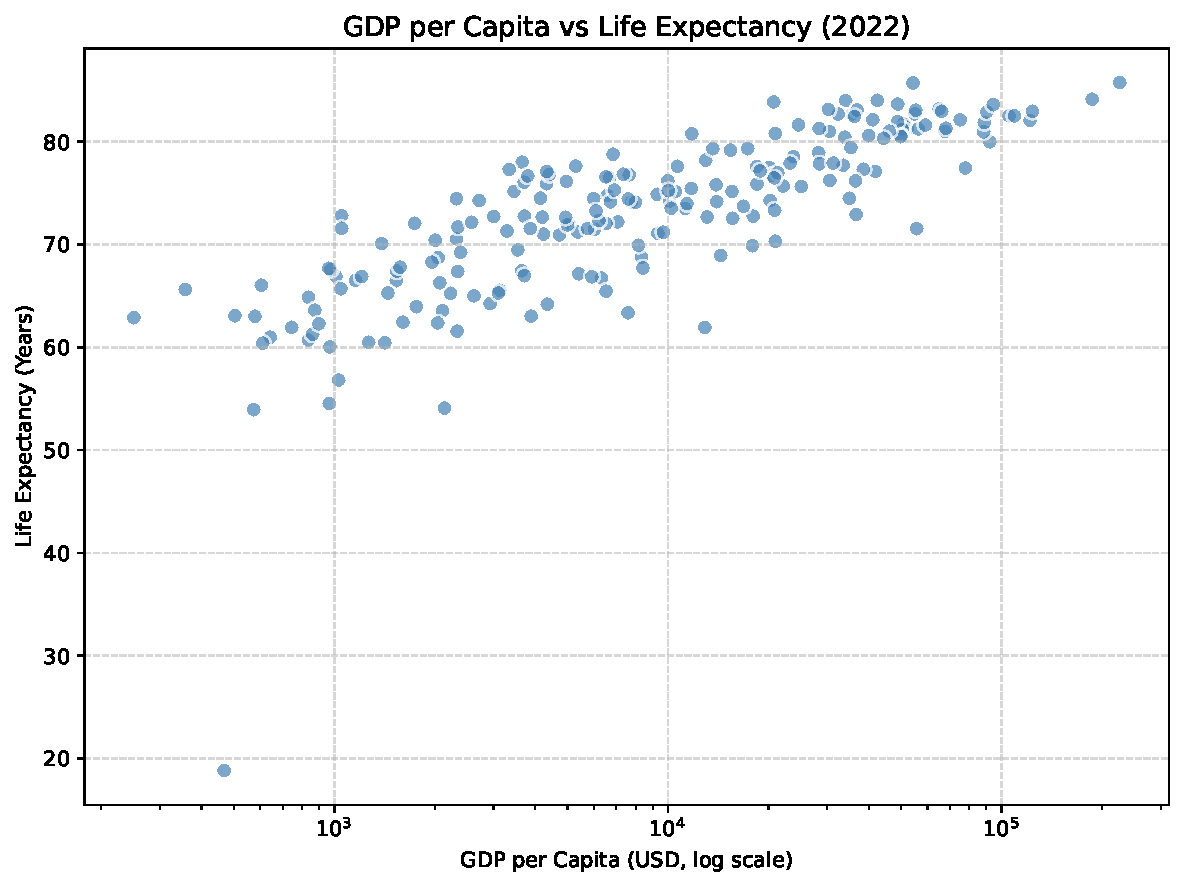
\includegraphics[keepaspectratio]{Assignment05_files/figure-pdf/fig-gdp-life-output-1.pdf}}

}

\caption{\label{fig-gdp-life}Relationship between GDP per Capita and
Life Expectancy (2022). Source: World Development Indicators, World
Bank.}

\end{figure}%

\emph{Relationship between GDP per Capita and Life Expectancy (2022).}

\emph{Source: World Development Indicators, World Bank.}

\textbf{Figure 1 Interpretation}: The scatter plot displays a strong
positive correlation between GDP per capita and life expectancy across
countries in 2022. As national income rises, citizens tend to live
longer --- reflecting improved access to healthcare, nutrition, and
living standards. However, the curve flattens for high-income nations,
suggesting diminishing marginal health benefits of additional income
once a country achieves a certain level of economic development.

\textbf{3.2 Education Expenditure by Country}

\begin{figure}

\centering{

\pandocbounded{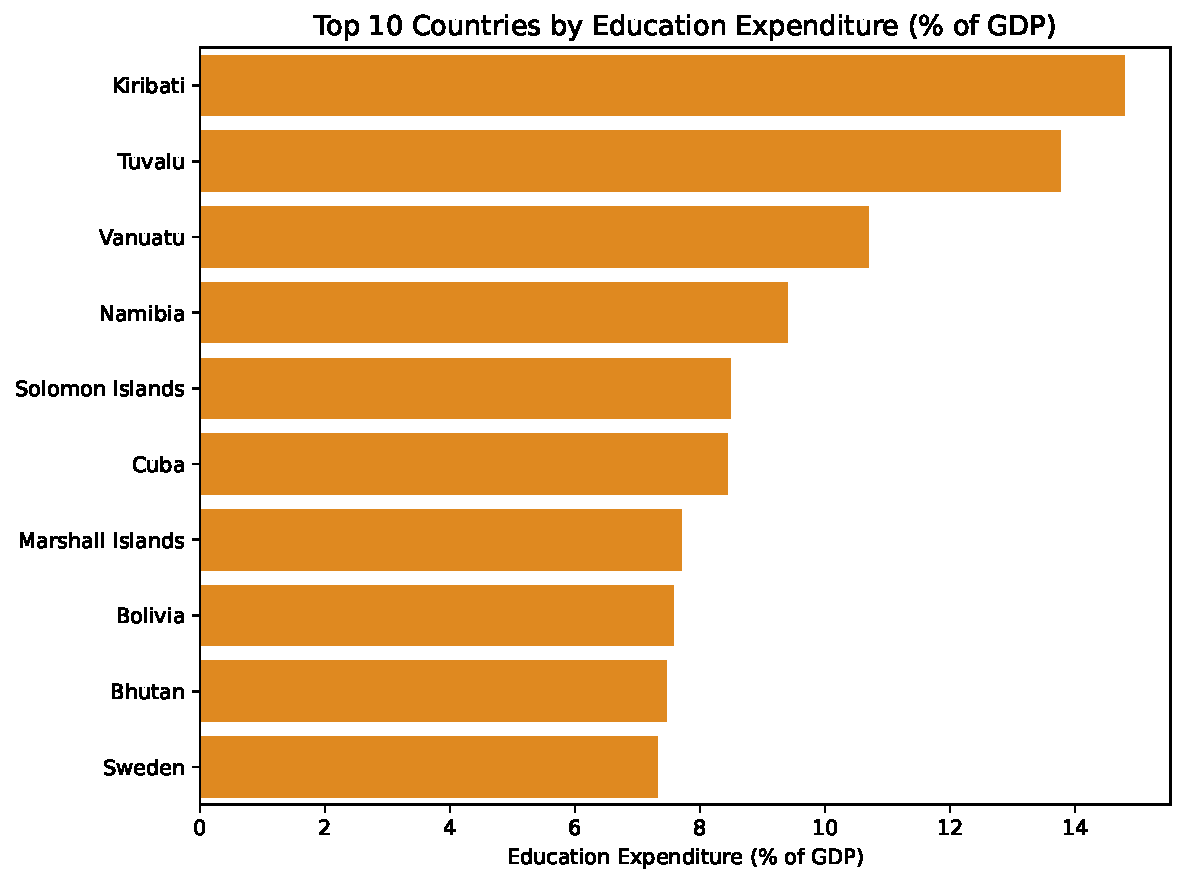
\includegraphics[keepaspectratio]{Assignment05_files/figure-pdf/fig-edu-top10-output-1.pdf}}

}

\caption{\label{fig-edu-top10}Top 10 Countries by Education Expenditure
as a Percentage of GDP (2022). Source: World Development Indicators,
World Bank.}

\end{figure}%

\emph{Top 10 Countries by Education Expenditure as a Percentage of GDP
(2022).}

\emph{Source: World Development Indicators, World Bank}

\textbf{Figure 2 interpretation}: The bar chart highlights the ten
countries investing the largest share of their GDP in education in 2022.
Small island nations such as Kiribati, Tuvalu, and Vanuatu lead the
list, each allocating over 10\% of their GDP to education --- far above
the global average of approximately 4\%. This trend reflects the
significant emphasis these nations place on human capital development
despite their limited economic scale. Larger economies like Sweden and
Cuba also appear on the list, demonstrating that both developed and
developing countries can prioritize education depending on their policy
objectives.

\begin{longtable}[]{@{}llll@{}}

\caption{\label{tbl-summary-stats}Summary Statistics for Key Development
Indicators (2022).}

\tabularnewline

\toprule\noalign{}
& gdp\_per\_capita & life\_expectancy &
education\_expenditure\_gdp\_share \\
\midrule\noalign{}
\endhead
\bottomrule\noalign{}
\endlastfoot
count & 208.00 & 217.00 & 163.00 \\
mean & 21175.31 & 73.11 & 4.26 \\
std & 31035.96 & 7.94 & 2.09 \\
min & 250.63 & 18.82 & 0.00 \\
25\% & 2692.57 & 67.79 & 2.90 \\
50\% & 7713.09 & 74.16 & 4.05 \\
75\% & 28905.93 & 78.53 & 5.24 \\
max & 226052.00 & 85.75 & 14.79 \\

\end{longtable}

\subsection{4. References}\label{references}

As shown in Figure~\ref{fig-gdp-life}, countries with higher GDP per
capita generally exhibit longer life expectancy. This relationship
reflects how income levels correlate with access to healthcare,
nutrition, and living standards.

Meanwhile, Figure~\ref{fig-edu-top10} highlights that several small
island nations allocate more than 10\% of their GDP to education --- a
significantly higher share compared to the global average of 4\%.

Finally, summary statistics presented in Table~\ref{tbl-summary-stats}
provide an overview of global variation across GDP, life expectancy, and
education expenditure, illustrating wide economic disparities.

According to the World Bank (Bank 2022), GDP per capita remains a
central indicator of economic development. Similarly, UNESCO data
(Statistics 2023) highlight that education spending varies widely by
region and income level.

\phantomsection\label{refs}
\begin{CSLReferences}{1}{0}
\bibitem[\citeproctext]{ref-worldbank2022}
Bank, World. 2022. {``World Development Indicators Database.''}
\url{https://databank.worldbank.org/source/world-development-indicators}.

\bibitem[\citeproctext]{ref-unesco2023}
Statistics, UNESCO Institute for. 2023. {``Education Expenditure as a
Share of GDP, 2023 Update.''}

\end{CSLReferences}




\end{document}
